\documentclass[12pt]{article}
\usepackage[margin=2.5cm]{geometry}
\usepackage{enumerate}
\usepackage{amsfonts}
\usepackage{amsmath}
\usepackage{fancyhdr}
\usepackage{amsmath}
\usepackage{amssymb}
\usepackage{amsthm}
\usepackage{mdframed}
\usepackage{graphicx}
\usepackage{subcaption}
\usepackage{listings}
\usepackage{xcolor}
\usepackage{booktabs}
\usepackage[utf]{kotex}

\definecolor{codegreen}{rgb}{0,0.6,0}
\definecolor{codegray}{rgb}{0.5,0.5,0.5}
\definecolor{codepurple}{rgb}{0.58,0,0.82}
\definecolor{backcolour}{rgb}{0.95,0.95,0.92}

\lstdefinestyle{mystyle}{
    backgroundcolor=\color{backcolour},
    commentstyle=\color{codegreen},
    keywordstyle=\color{magenta},
    numberstyle=\tiny\color{codegray},
    stringstyle=\color{codepurple},
    basicstyle=\ttfamily\footnotesize,
    breakatwhitespace=false,
    breaklines=true,
    captionpos=b,
    keepspaces=true,
    numbers=left,
    numbersep=5pt,
    showspaces=false,
    showstringspaces=false,
    showtabs=false,
    tabsize=1
}

\lstset{style=mystyle}

\begin{document}
\title{CSC148 Worksheet 7 Solution}
\author{Hyungmo Gu}
\maketitle

\section*{Question 1}

\begin{itemize}
    \item Noticed that there are 11 students in total.
    \item Students should be grouped by year as closest as possible.
\end{itemize}

\bigskip

\textbf{Notes:}

\begin{itemize}
    \item 형모 해낼 뚜 있쬬!
    \item 형모 화이팅!
\end{itemize}

\section*{Question 2}
\begin{center}
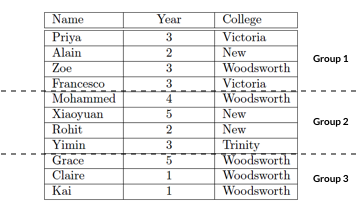
\includegraphics[width=0.7\linewidth]{images/worksheet_7_q2_solution.png}
\end{center}

\section*{Question 3}
\begin{itemize}
    \item

    First, we need to find the group as homogenous as possible in terms of year students
    are in.

    \bigskip

    The definition tells us group needs to be in 4,
    and the following table tell us there are 4 $3^{rd}$ year students.

    \bigskip

    \begin{center}
        \begin{tabular}{|c|c|}
            \hline
            Student Year & Number of Students\\
            \hline
            1 & 2\\
            \hline
            2 & 2\\
            \hline
            3 & 4\\
            \hline
            4 & 1\\
            \hline
            5 & 2\\
            \hline
        \end{tabular}
    \end{center}

    \bigskip

    It follows from these facts that the group of $3^{rd}$ year students best satisfy
    this criterion.

    \bigskip

    Next, we need to find the group as not homogenous as possible in terms of year students
    are in.

    \bigskip

    The same table tells us with 2 $5^{th}$ year students, 1 $4^{th}$
    year students and 1 $3^{rd}$ year student, a group spanning 3 years can be
    created.

    \bigskip

    Since we know there can't be a group spanning 4 years, we can conclude the
    group of 3 years (2 $5^{th}$ year students, 1 $4^{th}$ year students and 1
    $3^{rd}$ year student) best satisfy this criterion.

\end{itemize}

\bigskip

\begin{mdframed}
    \underline{\textbf{Correct Solution:}}

    \bigskip

    \color{red}
    Group 1 is the most homogeneous.

    \bigskip

    Group 3 is the least homogeneous.
    \color{black}

    \bigskip
\end{mdframed}

\bigskip

\section*{Question 4}
\begin{itemize}
    \item

    We will calculate the group score based on the code below. The code
    is also included in \textit{worksheet\_7\_q4\_solution.py}

    \bigskip

    \begin{lstlisting}[language=Python]
    def get_group_score(group):
        """Evaluates the group score

            Precondition: len(group) == 4
        """
        n = 4

        max_year = get_max_year(group)
        min_year = get_min_year(group)
        similarity_list = []

        i = 0

        while i < 4:
            j = 0
            while j < 4:
                # find the scaled distance
                scaled_distance = 0
                if max_year != min_year:
                    scaled_distance = abs(group[i]['year'] - group[j]['year']) / float(max_year - min_year)

                # find the similarity
                similarity = 1 - scaled_distance

                # add to list
                similarity_list.append(similarity)

                j += 1
            i += 1

        # find the average
        average = float(sum(similarity_list))/len(similarity_list)
        return average.as_integer_ratio()

    def get_max_year(group):
        """returns max value of year in group"""

        max_value = -1

        for student in group:
            max_value = max(student['year'], max_value)

        return max_value

    def get_min_year(group):
        """returns min value of year in group"""

        min_value = 100 # this is impossible value

        for student in group:
            min_value = min(student['year'], min_value)

        return min_value


    if __name__ == '__main__':
        group_1 = [{'name': 'Primya', 'year': 3},
        {'name': 'Zoe', 'year': 3},
        {'name': 'Francesco', 'year': 3},
        {'name': 'Yimin', 'year': 3}]

        group_2 = [{'name': 'Primya', 'year': 5},
        {'name': 'Zoe', 'year': 5},
        {'name': 'Francesco', 'year': 4},
        {'name': 'Yimin', 'year': 3}]


        score_1 =  get_group_score(group_1)
        print(score_1)

        score_2 =  get_group_score(group_2)
        print(score_2)


    \end{lstlisting}

    \bigskip

    For the most homogeneous group, the group score is 1.

    \bigskip

    For the least homogeneous group, the group score is $\frac{9}{16}$.

\end{itemize}

\bigskip

\begin{mdframed}
    \underline{\textbf{Correct Solution:}}

    \bigskip

    We will calculate the group score \color{red}using\color{black}\:the code below. The code
    is also included in \textit{worksheet\_7\_q4\_solution.py}

    \bigskip

    \begin{lstlisting}[language=Python]
    def get_similarity_list(group):
        """Evaluates the list of similarities""" # <- Correct solution
        similarity_list = []

        i = 0

        while i < len(group): # <- correct solution
            j = i + 1 # <- correct solution
            while j < len(group): # <- correct solution
                # find the scaled distance
                scaled_distance = abs(group[i]['year'] - group[j]['year']) / 5.0 # <- correct solution

                # find the similarity
                similarity = 1 - scaled_distance

                # add to list
                similarity_list.append(similarity)

                j += 1
            i += 1

        return similarity_list


    if __name__ == '__main__':
        # Correct Solution
        group_1 = [{'name': 'Primya', 'year': 3},
        {'name': 'Alain', 'year': 2},
        {'name': 'Zoe', 'year': 3},
        {'name': 'Francesco', 'year': 3}]

        # Correct Solution
        group_2 = [{'name': 'Mohammed', 'year': 4},
        {'name': 'Xiaoyuan', 'year': 5},
        {'name': 'Rohit', 'year': 2},
        {'name': 'Yimin', 'year': 3}]

        # Correct Solution
        group_3 = [{'name': 'Grace', 'year': 5},
        {'name': 'Claire', 'year': 1},
        {'name': 'Kai', 'year': 1}]

        # Correct Solution
        list_1 =  get_similarity_list(group_1)
        print(list_1)

        # Correct Solution
        list_2 =  get_similarity_list(group_2)
        print(list_2)

        # Correct Solution
        list_3 =  get_similarity_list(group_3)
        print(list_3)

    \end{lstlisting}

    \bigskip

    \color{red}
    We will calculate the score of each group in parts.

    \bigskip

    \underline{\textbf{Part 1 (Score of Group 1):}}

    \bigskip

    We need to calculate the score of group 1.

    \bigskip

    The problem tells us the group score is

    \begin{align}
        \text{Group Score} = \frac{\sum \text{similarities}}{\text{\# of elements in list of similarities}}
    \end{align}

    \bigskip

    and the above program tells us that the list of similarities are

    \begin{align}
        [0.8, 1.0, 1.0, 0.8, 0.8, 1.0]
    \end{align}

    \bigskip

    Then, using these facts, we can conclude that

    \begin{align}
        \text{Group Score} &= \frac{0.8 + 1.0 + 1.0 + 0.8 + 0.8 + 1.0}{6}\\
        &= \frac{\frac{4}{5} + 1 + 1 + \frac{4}{5} + \frac{4}{5} + 1}{6}\\
        &= \frac{\frac{4}{5} + \frac{5}{5} + \frac{5}{5} + \frac{4}{5} + \frac{4}{5} + \frac{5}{5}}{6}\\
        &= \frac{\frac{27}{4}}{6}\\
        &= \frac{27}{30}\\
        &= \frac{9}{10}
    \end{align}

    \bigskip

    \underline{\textbf{Part 2 (Score of Group 2):}}

    \bigskip

    We need to calculate the score of group 2.

    \bigskip

    The problem tells us the group score is

    \begin{align}
        \text{Group Score} = \frac{\sum \text{similarities}}{\text{\# of elements in list of similarities}}
    \end{align}

    \bigskip

    and the above program tells us that the list of similarities are

    \begin{align}
        [0.8, 0.6, 0.8, 0.4, 0.6, 0.8]
    \end{align}

    \bigskip

    Then, we can conclude that the value of group score is

    \begin{align}
        \frac{0.8 + 0.6 + 0.8 + 0.4 + 0.6 + 0.8}{6} &= \frac{\frac{4}{5} + \frac{3}{5} + \frac{4}{5} + \frac{2}{5} + \frac{3}{5} + \frac{4}{5}}{6}\\
        &= \frac{\frac{20}{5}}{6}\\
        &= \frac{20}{30}\\
        &= \frac{2}{3}
    \end{align}

    \bigskip

    \underline{\textbf{Part 3 (Score of Group 3):}}

    \bigskip

    We need to calculate the score of group 3.

    \bigskip

    The problem tells us the group score is

    \begin{align}
        \text{Group Score} = \frac{\sum \text{similarities}}{\text{\# of elements in list of similarities}}
    \end{align}

    \bigskip

    and the above program tells us that the list of similarities are

    \begin{align}
        [0.2, 0.2, 1.0]
    \end{align}

    \bigskip

    Then, we can conclude that the value of group score is

    \begin{align}
        \frac{0.2 + 0.2 + 1.0}{3} &= \frac{\frac{1}{5} + \frac{1}{5} + \frac{5}{5}}{3}\\
        &= \frac{\frac{7}{5}}{3}\\
        &= \frac{7}{15}
    \end{align}

    \color{black}
\end{mdframed}

\bigskip

\textbf{Notes:}

\begin{itemize}
    \item Realized that `group' in question means `group 1`, `group 2` and `group 3' in question 2 :(.
\end{itemize}

\bigskip

\section*{Question 5}
\begin{itemize}
    \item

    \bigskip

    We need to find the highest and the lowest possible score on this criterion.

    \bigskip

    We will do so in parts.

    \bigskip

    \underline{\textbf{Part 1 (Calculating highest possible group score):}}

    \bigskip

    We need to find the highest possible group score on this criterion.

    \bigskip

    The definition of group score tells us that

    \setcounter{equation}{0}
    \begin{align}
        \text{Group Score} = \frac{\displaystyle\sum\limits_{i=0}^{n-1} \displaystyle\sum\limits_{j=i+1}^{n-1} \left(1 - \displaystyle\frac{\lvert student\_year_i - student\_year_j \rvert}{5} \right)}{\text{\# of elements in list of similarities}}
    \end{align}

    \bigskip

    By observation, we can conclude that the highest possible group score happens when
    $\lvert student\_year_i - student\_year_j \rvert = 0$.

    \bigskip

    Then, using this fact, we can calculate that

    \begin{align}
        \text{Group Score} &= \frac{\displaystyle\sum\limits_{i=0}^{n-1} \displaystyle\sum\limits_{j=i+1}^{n-1} \left(1 - \displaystyle\frac{\lvert student\_year_i - student\_year_j \rvert}{5} \right)}{\text{\# of elements in list of similarities}}\\
        &= \frac{\displaystyle\sum\limits_{i=0}^{n-1} \displaystyle\sum\limits_{j=i+1}^{n-1} 1}{\text{\# of elements in list of similarities}}
    \end{align}

    \bigskip

    Then, because we know $\sum\limits_{i=0}^{n-1}\sum\limits_{j=i+1}^{n-1} 1 = \text{\# of elements in list of similarities}$,
    we can conclude

    \begin{align}
        &= \frac{\text{\# of elements in list of similarities}}{\text{\# of elements in list of similarities}}\\
        &= 1
    \end{align}

    \bigskip

    \underline{\textbf{Part 2 (Calculating lowest possible group score):}}

    \bigskip

    We need to find the lowest possible group score achievable on this criterion.

    \bigskip

    The definition of group score tells us that

    \begin{align}
        \text{Group Score} = \frac{\displaystyle\sum\limits_{i=0}^{n-1} \displaystyle\sum\limits_{j=i+1}^{n-1} \left(1 - \displaystyle\frac{\lvert student\_year_i - student\_year_j \rvert}{5} \right)}{\text{\# of elements in list of similarities}}
    \end{align}

    \bigskip

    By observation, we can conclude that the lowest possible group score happens when
    $\lvert student\_year_i - student\_year_j \rvert = 5$.

    \bigskip

    Then, using this fact, we can calculate that

    \begin{align}
        \text{Group Score} &= \frac{\displaystyle\sum\limits_{i=0}^{n-1} \displaystyle\sum\limits_{j=i+1}^{n-1} \left(1 - \displaystyle\frac{\lvert student\_year_i - student\_year_j \rvert}{5} \right)}{\text{\# of elements in list of similarities}}\\
        &= \frac{\displaystyle\sum\limits_{i=0}^{n-1} \displaystyle\sum\limits_{j=i+1}^{n-1} 0}{\text{\# of elements in list of similarities}}\\
        &= \frac{0}{\text{\# of elements in list of similarities}}\\
        &= 0
    \end{align}
\end{itemize}

\bigskip

\textbf{Notes:}

\begin{itemize}
    \item 형모야. 차분히. 한걸음 더.
    \item 문제 안풀린다고 주저 앉지마.
    \item 사랑하는 내 여보 향해 가는거야.
    \item 보고싶은 내 여보 향해.
    \item 형모야 화이팅 :)
\end{itemize}

\section*{Question 6}

\begin{center}
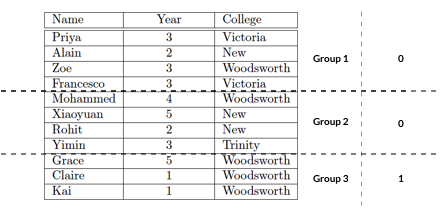
\includegraphics[width=0.7\linewidth]{images/worksheet_7_q6_solution.png}
\end{center}

\section*{Question 7}
\begin{itemize}
    \item

    We need to evaluate the total score for each group.

    \bigskip

    We will do so in parts.

    \bigskip

    \underline{\textbf{Part 1 (Calculating the total score of Group 1):}}

    \bigskip

    We need to calculate the total score of group 1.

    \bigskip

    The answer from question 4 tells us group 1 has value of $\frac{9}{10}$, and
    for criterion a) and has $0$ for criterion b).

    \bigskip

    Since we know criterion a) has weight of $0.8$ and criterion has weight of $0.2$,
    we can conclude the total score is

    \setcounter{equation}{0}
    \begin{align}
        (0.8 \times \frac{9}{10}) + (0.2 \times 0 ) &= 0.72\\
        &\approx 1
    \end{align}

    \bigskip

    \underline{\textbf{Part 2 (Calculating the total score of Group 2):}}

    \bigskip

    We need to calculate the total score of group 2.

    \bigskip

    The answer from question 4 tells us group 2 has value of $\frac{2}{3}$, and
    for criterion a) and has $0$ for criterion b).

    \bigskip

    Since we know criterion a) has weight of $0.8$ and criterion has weight of $0.2$,
    we can conclude the total score is

    \begin{align}
        (0.8 \times \frac{2}{3}) + (0.2 \times 0 ) &= 0.5333333\\
        &\approx 1
    \end{align}

    \underline{\textbf{Part 3 (Calculating the total score of Group 3):}}

    \bigskip

    We need to calculate the total score of group 3.

    \bigskip

    The answer from question 4 tells us group 3 has value of $\frac{7}{15}$, and
    for criterion a) and has $1$ for criterion b).

    \bigskip

    Since we know criterion a) has weight of $0.8$ and criterion has weight of $0.2$,
    we can conclude the total score is

    \begin{align}
        (0.8 \times \frac{7}{15}) + (0.2 \times 1 ) &= 0.573333\\
        &\approx 1
    \end{align}

\end{itemize}

\bigskip

\begin{mdframed}
    \underline{\textbf{Correct Solution:}}

    \bigskip

    We need to evaluate the total score for each group.

    \bigskip

    We will do so in parts.

    \bigskip

    \underline{\textbf{Part 1 (Calculating the total score of Group 1):}}

    \bigskip

    We need to calculate the total score of group 1.

    \bigskip

    \color{red}
    The formula for total score tells us
    \setcounter{equation}{0}
    \begin{align}
        \text{Total Score} &= (\text{Score of Criterion a} \times 80) + (\text{Score of Criterion b} \times 20)
    \end{align}
    \color{black}

    \bigskip

    Since we know \color{red}group 1 has score of $\frac{9}{10}$ for criteron a) and score of $0$ for
    criterion b)\color{black}, we can conclude the total score is

    \color{red}
    \begin{align}
        (\frac{9}{10} \times 80) + (0 \times 20) &= 72
    \end{align}
    \color{black}

    \bigskip

    \underline{\textbf{Part 2 (Calculating the total score of Group 2):}}

    \bigskip

    We need to calculate the total score of group 2.

    \bigskip

    \color{red}
    The formula for total score tells us

    \begin{align}
        \text{Total Score} &= (\text{Score of Criterion a} \times 80) + (\text{Score of Criterion b} \times 20)
    \end{align}
    \color{black}

    \bigskip

    Since we know \color{red}group 2 has score of $\frac{2}{3}$ for criteron a) and score of $0$ for
    criterion b)\color{black}, we can conclude the total score is

    \color{red}
    \setcounter{equation}{0}
    \begin{align}
        (\frac{2}{3} \times 80) + (0 \times 20) &= 53.33333\\
        &\approx 53
    \end{align}
    \color{black}

    \underline{\textbf{Part 3 (Calculating the total score of Group 3):}}

    \bigskip

    We need to calculate the total score of group 3.

    \bigskip

    \color{red}
    The formula for total score tells us

    \begin{align}
        \text{Total Score} &= (\text{Score of Criterion a} \times 80) + (\text{Score of Criterion b} \times 20)
    \end{align}
    \color{black}

    \bigskip

    Since we know \color{red}group 3 has score of $\frac{7}{15}$ for criteron a) and score of $1$ for
    criterion b)\color{black}, we can conclude the total score is

    \color{red}
    \setcounter{equation}{0}
    \begin{align}
        (\frac{7}{15} \times 80) + (1 \times 20) &= 57.33333\\
        &\approx 57
    \end{align}
    \color{black}

\end{mdframed}

\section*{Question 8}

\bigskip

\begin{itemize}
    \item

    We need to calculate the lowest and highest possible total score.

    \bigskip

    We will do so in parts.

    \bigskip

    \underline{\textbf{Part 1 (Calculating the highest possible total score):}}

    \bigskip

    We need to calculate the highest possible total score.

    \bigskip

    The formula for total score tells us that

    \setcounter{equation}{0}
    \begin{align}
        \text{Total Score} &= (\text{Score of Criterion a} \times 80) + (\text{Score of Criterion b} \times 20)
    \end{align}

    \bigskip

    By observation, we can conclude the maximum total score occurs when Score of Criterion a
    and Score of Criterion b are both at maximum.

    \bigskip

    Because we know the maximum possible score for criterion a and b are 1,
    we can conclude the maximum possible total score is

    \begin{align}
        \text{Total Score} &= (1 \times 80) + (1 \times 20)\\
        &= 100
    \end{align}

    \bigskip

    \underline{\textbf{Part 2 (Calculating the lowest possible total score):}}

    \bigskip

    We need to calculate the lowest possible total score.

    \bigskip

    The formula for total score tells us that

    \begin{align}
        \text{Total Score} &= (\text{Score of Criterion a} \times 80) + (\text{Score of Criterion b} \times 20)
    \end{align}

    \bigskip

    By observation, we can conclude the minimum total score occurs when Score of Criterion a
    and Score of Criterion b are both at minimum.

    \bigskip

    Because we know the minimum possible score for criterion a and b are 0,
    we can conclude the minimum possible total score is

    \begin{align}
        \text{Total Score} &= (0 \times 80) + (0 \times 20)\\
        &= 0
    \end{align}

\end{itemize}

\bigskip

\begin{mdframed}
    \underline{\textbf{Rough Work:}}

    \bigskip

    We need to calculate the lowest and highest possible total score.

    \bigskip

    We will do so in parts.

    \bigskip

    \underline{\textbf{Part 1 (Calculating the highest possible total score):}}

    \bigskip

    We need to calculate the highest possible total score.

    \bigskip

    \begin{itemize}
        \item State the formula

        \begin{mdframed}
        The formula for total score tells us that

        \begin{align}
            \text{Total Score} &= (\text{Score of Criterion a} \times 80) + (\text{Score of Criterion b} \times 20)
        \end{align}
        \end{mdframed}

        \item Show the maximum occurs when score of criterion a and score of criterion b is maximum

        \begin{mdframed}
        By observation, we can conclude the maximum total score occurs when Score of Criterion a
        and Score of Criterion b are both at maximum.
        \end{mdframed}

        \item Calculate maximum possible total score using the fact 1 is the highest possible score
        for both criterion a and criterion b.

        \begin{mdframed}
        Because we know the maximum possible score for criterion a and b are 1,
        we can conclude the maximum possible total score is

        \begin{align}
            \text{Total Score} &= (1 \times 80) + (1 \times 20)\\
            &= 100
        \end{align}

        \end{mdframed}
    \end{itemize}

    \bigskip

    \underline{\textbf{Part 2 (Calculating the lowest possible total score):}}

    \bigskip

    We need to calculate the lowest possible total score.

    \bigskip

    \begin{itemize}
        \item State the formula
        \begin{mdframed}
        The formula for total score tells us that

        \begin{align}
            \text{Total Score} &= (\text{Score of Criterion a} \times 80) + (\text{Score of Criterion b} \times 20)
        \end{align}
        \end{mdframed}

        \item Show the minimum occurs when score of criterion a and score of criterion b is minimum

        \begin{mdframed}
        By observation, we can conclude the minimum total score occurs when Score of Criterion a
        and Score of Criterion b are both at minimum.
        \end{mdframed}

        \item Calculate minimum possible total score using the fact 1 is the highest possible score
        for both criterion a and criterion b.

        \begin{mdframed}
            Because we know the minimum possible score for criterion a and b are 0,
            we can conclude the minimum possible total score is

            \begin{align}
                \text{Total Score} &= (0 \times 80) + (0 \times 20)\\
                &= 0
            \end{align}
        \end{mdframed}
    \end{itemize}
\end{mdframed}

\section*{Question 9}

\bigskip

\begin{itemize}
    \item

    We need to compute the average score across all the groups.

    \bigskip

    The formula for average total score tells us

    \setcounter{equation}{0}
    \begin{align}
        \text{Average Total Score} = \frac{\sum\limits_{i} \text{Total Score of Group } i}{\text{\# of Groups}}
    \end{align}

    \bigskip

    Using the fact there are 3 groups with the total score of 72 for group 1,
    53 for group 2, and 57 for group 3, we can calculate

    \begin{align}
        \text{Average Total Score} &= \frac{72 + 53 + 57}{3}\\
        &= \frac{182}{3}\\
        &\approx 60.667
    \end{align}
\end{itemize}

\bigskip

\begin{mdframed}
    \underline{\textbf{Rough Work:}}

    \bigskip

    We need to compute the average score across all the groups.

    \bigskip

    \begin{itemize}
        \item State the formula of average total score
        \begin{mdframed}
            The formula for average total score tells us

            \begin{align}
                \text{Average Total Score} = \frac{\sum\limits_{i} \text{Total Score of Group } i}{\text{\# of Groups}}
            \end{align}
        \end{mdframed}

        \item Show the average total score using the fact group 1 has total score of 72,
        group 2 has total score of 53 and group 3 has total score of 57.

        \begin{mdframed}
            Using the fact there are 3 groups with the total score of 72 for group 1,
            53 for group 2, and 57 for group 3, we can calculate

            \begin{align}
                \text{Average Total Score} &= \frac{72 + 53 + 57}{3}\\
                &= \frac{182}{3}\\
                &\approx 60.667
            \end{align}
        \end{mdframed}
    \end{itemize}

\end{mdframed}

\section*{Question 10}

\bigskip

\begin{mdframed}
    \underline{\textbf{Rough Work:}}

    \bigskip

    We need to find the 3 groups that results in the better average total score
    than 60.667.

    \bigskip

    \begin{itemize}
        \item State the alternate 3 groups

        \begin{mdframed}
        Consider the following 3 groups.

        \bigskip

        \begin{center}
            \centering
            \begin{tabular}{|p{2.5cm}|p{2.5cm}|p{2.5cm}|}
                \hline
                \multicolumn{3}{|c|}{\textbf{Group 1}}\\
                \hline
                Name & Year & College\\
                \hline
                Priya & 3 & Victoria\\
                \hline
                Zoe & 3 & Woodsworth\\
                \hline
                Francesco & 3 & Victoria\\
                \hline
                Yimin & 3 & Trinity\\
                \hline
            \end{tabular}

            \bigskip

            \begin{tabular}{|p{2.5cm}|p{2.5cm}|p{2.5cm}|}
                \hline
                \multicolumn{3}{|c|}{\textbf{Group 2}}\\
                \hline
                Name & Year & College\\
                \hline
                Alain & 2 & New\\
                \hline
                Rohit & 2 & New\\
                \hline
                Claire & 1 & Woodsworth\\
                \hline
                Kai & 1 & Woodsworth\\
                \hline
            \end{tabular}

            \bigskip

            \begin{tabular}{|p{2.5cm}|p{2.5cm}|p{2.5cm}|}
                \hline
                \multicolumn{3}{|c|}{\textbf{Group 3}}\\
                \hline
                Name & Year & College\\
                \hline
                Mohammed & 4 & Woodsworth\\
                \hline
                Xiaoyuan & 5 & New\\
                \hline
                Grace & 5 & Woodsworth\\
                \hline
            \end{tabular}
        \end{center}


        \end{mdframed}
        \item Show the group score of each group, using the same steps from
        question 4
        \item Show the total score of each group
        \item Show the average total score of the 3 groups is higher than
        60.667
    \end{itemize}


\end{mdframed}

\end{document}